%% Project report — 3D all-sky monochromatic radiative transfer (rt3d)
%% Build: latexmk -pdf main.tex   (TeX Live)
%% Figures + table fragments are generated by scripts/report_figures.py
\documentclass[11pt,a4paper]{article}

\usepackage[T1]{fontenc}
\usepackage[utf8]{inputenc}
\usepackage{lmodern}
\usepackage[margin=2.4cm]{geometry}
\usepackage{graphicx}
\graphicspath{{figures/}}
\usepackage{booktabs}
\usepackage{array}
\usepackage{amsmath,amssymb}
\usepackage{microtype}
\usepackage{caption}
\usepackage{float}
\usepackage{tikz}
\usepackage{xcolor}
\usepackage[pdfusetitle,hidelinks]{hyperref}

\usetikzlibrary{arrows.meta,positioning,fit,backgrounds,shapes.geometric}

\captionsetup{font=small,labelfont=bf}
\setlength{\parskip}{0.4em}

\newcommand{\ke}{\kappa_e}
\newcommand{\ks}{\kappa_s}
\newcommand{\ka}{\kappa_a}
\newcommand{\Om}{\Omega}
\newcommand{\dg}{\mathrm{dg}}

\title{\texorpdfstring{\bfseries A three-dimensional all-sky monochromatic
radiative-transfer solver\\[0.4em]
\large Short characteristics on an octree, Monte Carlo cross-validation,
and a pinned regression gate\\[0.6em]
\normalsize Project report --- \texttt{rt3d} code base, branch \texttt{main}}
{A three-dimensional all-sky monochromatic radiative-transfer solver:
short characteristics on an octree, Monte Carlo cross-validation,
and a pinned regression gate}}
\author{\texttt{3d\_rt} radiative-transfer project}
\date{November 16, 2026}

\begin{document}
\maketitle

\begin{abstract}
\noindent
This report documents \texttt{rt3d}, a three-dimensional scalar
radiative-transfer solver for an all-sky scene: a cuboid domain with
periodic side walls, open top, and a flat Lambertian/emissive ground,
illuminated by a direct solar beam and embedded in a participating medium
of spatially varying extinction, scattering coefficient, asymmetry
parameter, and temperature. The formulation is monochromatic and local
(LTE): absorption and Henyey--Greenstein scattering with a local source
$S=(1-\omega_s)B+\omega_s J$. Two independent solver families are
implemented and cross-validated: a short-characteristics (SC) family with
an octree spatial grid, exact characteristic marches, and a
lambda-iteration/Ng-accelerated iteration loop; and a Monte Carlo (MC)
family with Woodcock null-collision tracking, a two-stage forward solver,
and a backward (adjoint) solver. All results rest on five verification invariants
and a six-tier cross-solver test matrix in which every accepted
imperfection is pinned as a measured regression band. Fourteen findings
(F1--F14) document what the numbers mean: two real bugs fixed during the
campaign (F12, F13), several structural error floors (F11 unigrid
grazing-ray error, F14 direction-quadrature beam mismatch), and rules
for reading MC statistics honestly (F3, F9). All figures in this report
are generated from the same solves the pytest gate pins.
\end{abstract}

\tableofcontents

%=============================================================================
\section{Introduction}
%=============================================================================

\texttt{rt3d} solves the scalar radiative-transfer equation (RTE) in a
three-dimensional, inhomogeneous, scattering--absorbing medium under
all-sky illumination. The design goals, in priority order, were:
(i)~\emph{correctness under scrutiny} --- every transport path is validated
against analytic limits and against an independent solver family, and every
residual defect is pinned as a measured regression band rather than
silently tolerated;
(ii)~\emph{geometric adaptivity} --- an octree driven by local optical
depth so that resolution is spent where the cloud is;
(iii)~\emph{algorithmic independence} --- a deterministic SC family and a
statistical MC family that share only the geometry and input sampling, so
that agreement between them is strong evidence.

The scope assumptions are fixed by design (they are \emph{not} incidental):
monochromatic (one frequency at a time, no line structure), LTE with a
local source function, no polarization (scalar RTE only; the Stokes
machinery in the legacy \texttt{scripts/icosphere\_grid.py} is unused),
straight rays (no refraction), a collimated solar beam, periodicity in
$x$ and $y$, and Henyey--Greenstein (HG) scattering. The spatial
discretization is an extinction-driven octree; the angular discretization
is an icosahedral geodesic grid; the iteration is lambda iteration with
one-dimensional Ng acceleration, structured like the DOIT solver of ARTS.

The repository contains the solver package (\texttt{rt3d/}, including the
Monte Carlo family \texttt{rt3d/mc/}), a pytest cross-solver test matrix
(\texttt{tests/test\_matrix\_*.py}: 135 tests in the tiers T0--T5 plus the
MC-ground suite M6) and per-feature suites for individual components ---
341 tests collected in total --- plus standalone research runners
(\texttt{scripts/}). Roughly 24\,500 lines of Python cover solver,
tests, and scripts. The environment is a pinned miniforge environment
(\texttt{pyarts}): Python 3.14.6, NumPy 2.5.2, SciPy 1.18.0,
matplotlib 3.11.1, Numba 0.66.0 (JIT on Python 3.14), pytest 9.1.1; every
JIT fast path has a pure-NumPy reference fallback and both must agree
bit-identically (tier T1).

\emph{How to read this report.} Sections~\ref{sec:formulation}--\ref{sec:iteration}
describe the physics and the two solver families; section~\ref{sec:validation}
describes the validation architecture (invariants, tiers, pinned bands);
section~\ref{sec:results} presents the measured results and the findings
F1--F14 that govern their interpretation; section~\ref{sec:performance}
covers performance; section~\ref{sec:conclusions} states limitations.
Every figure is regenerable end-to-end with the commands in
appendix~\ref{sec:reproduce}; the scalar numbers quoted in the text are the
same ones the pytest gate pins.

%=============================================================================
\section{Physical formulation}
\label{sec:formulation}
%=============================================================================

\subsection{Transport equation and inputs}

For a monochromatic intensity $I(\mathbf r,\Om)$ along direction $\Om$,
\begin{equation}
\Om\cdot\nabla I + \ke\, I
\;=\; \ks\!\int \Phi_{\mathrm{HG}}(\Om'\to\Om)\, I(\Om')\,d\Om'
\;+\; \ka\, B(\mathbf r),
\label{eq:rte}
\end{equation}
with derived quantities computed, never stored,
\begin{equation}
\ka=\ke-\ks,\qquad
\omega_s=\ks/\ke\ \ (\text{guarded as } \ke\to0),\qquad
\Phi_{\mathrm{HG}}(\Theta)=\frac{1-g^2}{4\pi\,\bigl(1+g^2-2g\cos\Theta\bigr)^{3/2}} .
\end{equation}
The four physical inputs are the extinction coefficient $\ke$, the
scattering coefficient $\ks$, the temperature $T$ (through the Planck
function $B$), and the asymmetry parameter $g$; the older convention of
storing an albedo is not used. The report case (\texttt{gaussian\_cloud}
case, the MANUAL \S11 worked example) places a normalized Gaussian cloud
in a $10\times10\times10$\,m periodic box with $\omega_s\le0.9$
($\omega_{\mathrm{cap}}=0.9$), $g\le0.925$, and optical depth
$\tau\approx2$ through the core.

\subsection{Solar beam split}

The direct beam is a delta in direction and cannot live on an angular
quadrature, so the solver splits $I=I_{\mathrm{diff}}+I_{\mathrm{beam}}$:
a dedicated sweep provides the beam optical depth $\tau_b(\mathbf r)$
along $\Om_{\odot}$ (exact to machine precision, invariant~3; the case uses
a $30^\circ$ solar zenith), giving $I_{\mathrm{beam}}=F_0\,
e^{-\tau_b}$, and the beam's \emph{first-scattering} contribution
$\ks\,\Phi_{\mathrm{HG}}(\Om_\odot\to\Om_i)\,F_0\,e^{-\tau_b}$ enters the
source function as a fixed term that is never iterated on the
quadrature. The beam is reflected at the ground in the same Lambertian
way as the diffuse field. (The precise normalization convention of the
first-scatter term differs between the two families and is finding F14,
section~\ref{sec:findings}.)

\subsection{Boundary conditions}

\begin{itemize}
\item \textbf{Top}: $I_{\mathrm{diff}}=$ const (case: $I=1$); space above.
\item \textbf{Bottom}: flat ground at $z=z_0$ with a Lambertian, emissive
law
\begin{equation}
I_{\uparrow} \;=\; \frac{A_g}{\pi}\,F_{\downarrow}
\;+\; \varepsilon_g\,B(T_g),
\label{eq:ground}
\end{equation}
computed by sweeping the downward ordinates (and the analytic beam
irradiance) first; the case uses $A_g=0.3$, $\varepsilon_g=1$, $B_g=1$.
A hook for a variable-height surface exists in the SC family but raises
\texttt{NotImplementedError} in both families --- the only unsupported
configuration in the matrix.
\item \textbf{Sides}: periodic in $x$ and $y$ by wrapping ray exit to
entry. No ordinate is allowed exactly $\Om_z=0$ (such ordinates would
form cyclic characteristics under periodicity); the direction grid is
rotated on construction to guarantee this.
\end{itemize}

%=============================================================================
\section{Discretization}
\label{sec:discretization}
%=============================================================================

\subsection{Angular discretization: icosahedral grids with true solid angles}
\label{sec:dirs}

The direction grid is always an icosahedral (geodesic) grid with
$N_{\mathrm{dir}}=10\cdot4^{n_{\mathrm{refine}}}+2$ ordinates and
solid-angle weights $w_i$ obtained from spherical-triangle areas
(L'Huilier's formula distributed to vertices) --- never the equal-area
approximation $4\pi/N$, because icosphere vertices are not equal-area
(Fig.~\ref{fig:directions}). The \emph{development grid} for all
development, cases, benchmarks, and validation is
$n_{\mathrm{refine}}=1$ with 42 ordinates; $n_{\mathrm{refine}}$ is a
first-class configuration option (solver config, every case, every runner,
recorded in every output file), and nothing in the code may assume a
specific $N_{\mathrm{dir}}$. The refinement of the legacy icosphere code
was replaced by a vectorized, edge-indexed implementation so that the
convergence levels 162 and 642 are reachable.

\begin{figure}[htbp]
\centering
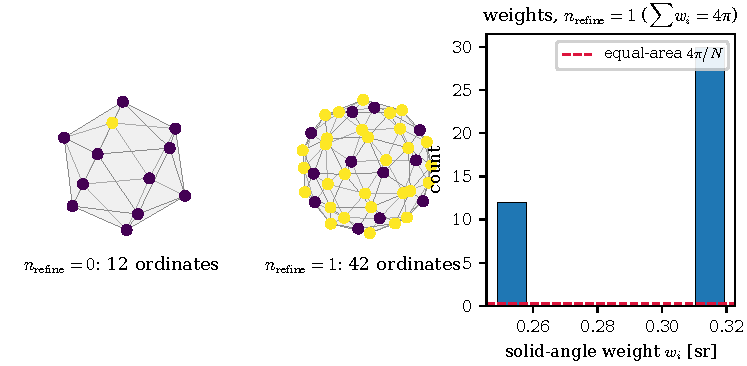
\includegraphics[width=.95\textwidth]{fig_directions.pdf}
\caption{Icosahedral direction grids: 12 and 42 ordinates as geodesic
triangulations with vertex markers colored by the solid-angle weight $w_i$;
panel (c): the weight distribution for $N_{\mathrm{dir}}=42$, showing why
$4\pi/N$ (dashed) is a poor approximation --- the weights span a factor
of about 1.3. Weights sum to $4\pi$ to machine precision (invariant~1).}
\label{fig:directions}
\end{figure}

The full-angle scattering integral becomes one BLAS matmul per iteration:
a precomputed matrix $\Phi_{ij}=\Phi_{\mathrm{HG}}(\Om_j\to\Om_i)$ of size
$N_{\mathrm{dir}}\times N_{\mathrm{dir}}$ is applied to all cells as
$(n_{\mathrm{cells}}\times N_{\mathrm{dir}})\;\Phi^{\mathsf T}$. When $g$
varies spatially (it does in the cloud case), cells are bucketed by $g$
and one matmul is performed per bucket. For $\delta$-M, the
$\delta$-matrix weights are built per $g$-bucket from the analytic HG
moments $g^n$ (Wiscombe).

\subsection{Spatial discretization: the octree}
\label{sec:octree}

The medium is meshed by a flat struct-of-arrays octree (cubic cells, 2:1
balance, maximum-depth cap). Refinement is driven by the \emph{input}
extinction: a cell splits when either its optical depth across the cell
exceeds a tolerance, $\ke\,h > \tau_{\max}$ (the accuracy-relevant measure
for short characteristics), or its internal extinction gradient is large,
$(\max\ke-\min\ke)/\overline{\ke}>\epsilon$ (cloud-edge resolution).
Per leaf, cell averages of $\ke,\ks,g,T$ are sampled from analytic
callables or from the interpolator fields of the legacy code. Point
location is $O(1)$ through a per-level lattice table. The base cell size
$h_0$ matters: refinement only adds leaves where the medium is, so
boundary faces keep base-size leaves and $h_0$ --- not the depth ---
controls anything evaluated on a face (finding F7).

\begin{figure}[htbp]
\centering
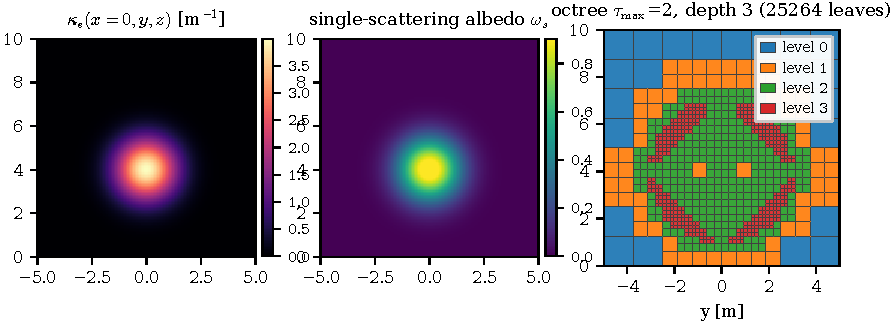
\includegraphics[width=.98\textwidth]{fig_octree.pdf}
\caption{Left: cloud-case input fields $\ke$ and $\omega_s$ on the plane
$x=0$ (the cloud: Gaussian core, $\omega_s\le0.9$, $g\le0.925$,
$\tau\approx2$). Right: octree leaves crossing the same plane for
$\tau_{\max}=2$, max depth 3 (25\,264 leaves), colored by level ---
resolution concentrates at the cloud, vacuum keeps base cells
($h_0=1.25$\,m). The reference rung of the test matrix uses
$\tau_{\max}=0.5$, depth 5: 50\,380 leaves.}
\label{fig:octree}
\end{figure}

The matrix ladder uses three octree knobs that are \emph{not}
interchangeable (F10): the $\tau_{\max}$ ladder runs at non-binding depth,
a depth ladder saturates, and $h_0$ barely moves cell-centered fields
while moving face quantities.

%=============================================================================
\section{Short-characteristics transport}
\label{sec:transport}
%=============================================================================

For each ordinate $\Om$, one characteristic passes through each cell or
leaf center. The solver implements three transport schemes over two grid
types, plus a legacy reference chain for the octree; all share the same
formal solution and boundary handling.

\subsection{Unigrid: lattice stencil chains}

For a Cartesian grid and direction $\Om$, a \emph{stencil}
$\mathbf s\in\mathbb Z^3$ is selected that minimizes the angle between
$\mathbf s\cdot h$ and $\Om$ among lattice candidates up to a radius
that scales with $\max(h)/\min(h)$ (Fig.~\ref{fig:stencil}, left). The
parent of a cell $c$ is $c-\mathbf s$; walking parents defines
characteristic chains. Because the ray direction and the stencil
direction differ slightly, each parent-to-center segment is split into
\emph{explicit sub-segments} --- exact crossings of cell boundaries along
the straight path --- so the formal solution accumulates optical depth
through the true crossed cells (Fig.~\ref{fig:stencil}, right and
Fig.~\ref{fig:subsegments}). This is what makes the chain exact in the
pure-absorber limit (left panel of Fig.~\ref{fig:beerk}): the swept
intensity matches $I_{\mathrm{entry}}\,e^{-\ke \ell}$ to floating-point
precision for all 42 ordinates.

Sweeps are executed by topological waves over chain depth: within a wave
all cells read their parents from the previous wave, so each wave is one
vectorized gather-scatter batch. Roots (chain heads) are closed by an
exact backward march to the entry face, where the boundary condition
(face inflow, periodic wrap, or ground radiance) supplies the entry
value. The second unigrid scheme, \emph{SC stencil}, uses a short
two-segment stencil instead of a full chain; it is cheaper but carries a
direction-dependent transport error (finding F11, right panel of
Fig.~\ref{fig:beerk}).

\begin{figure}[htbp]
\centering
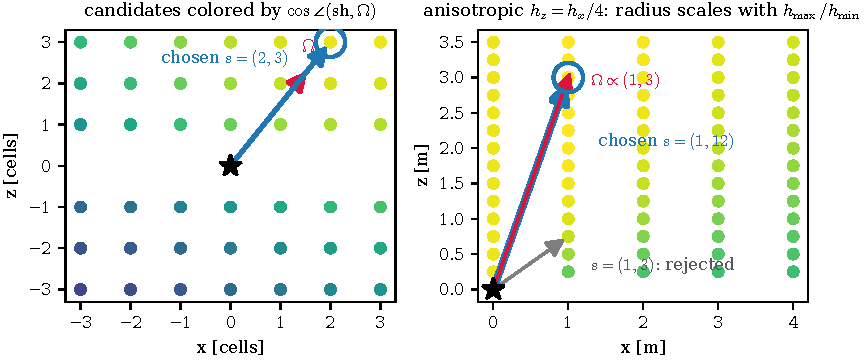
\includegraphics[width=.85\textwidth]{fig_stencil.pdf}
\caption{Stencil selection for a unigrid characteristic. Left: candidate
lattice offsets (colored by $\cos$ angle to $\Om$) and the chosen
stencil. Right: anisotropic cells ($h_z=h_x/4$) require a search radius
scaled by $h_{\max}/h_{\min}$ --- the naive short stencil points in a
badly wrong direction and is rejected.}
\label{fig:stencil}
\end{figure}

\begin{figure}[htbp]
\centering
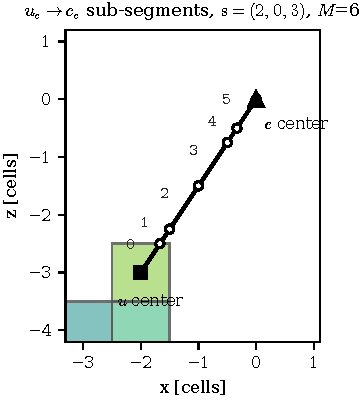
\includegraphics[width=.45\textwidth]{fig_subsegments.pdf}
\caption{Sub-segment splitting of one characteristic segment
($\mathbf s=(2,0,3)$): the straight path from parent center to target
center is cut at every crossed cell face; each sub-segment records
(cell, length), so optical depth is accumulated through the true
geometry even when the stencil direction is not the ray direction.}
\label{fig:subsegments}
\end{figure}

\subsection{Octree: exact backward marches}

On the octree the stencil notion is abandoned: for each leaf center the
solver performs an exact ray march backwards along $-\Om$ through the
tree (DDA), recording the traversed leaves and their segment lengths
down to the domain entry (or, for ground-fed ordinates, to the ground
entry cell after periodic wrapping, finding F13). Segments are stored in
a ray-contiguous layout (all segments of one ray adjacent, ordered center
$\to$ entry); per-ray prefix optical depths within a segment array are
obtained by a single cumulative sum corrected per block, so the whole
sweep stays vectorized (Fig.~\ref{fig:march}). The march is exact in the
pure-absorber limit to $10^{-15}$ relative (invariant~3 per family).

\begin{figure}[htbp]
\centering
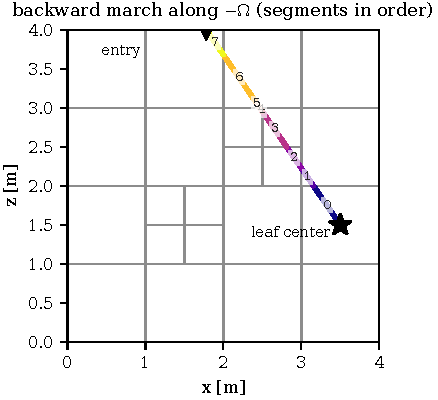
\includegraphics[width=.47\textwidth]{fig_octree_march.pdf}
\caption{One exact backward march from a leaf center along $-\Om$ through
a refined octree (2--D slice; segment numbers in traversal order). Mixed
leaf sizes are traversed exactly: unlike a stencil chain, the march
records the true sub-segment sequence across level boundaries.}
\label{fig:march}
\end{figure}

\subsection{\texorpdfstring{$\delta$-M}{delta-M} and beam optics}

The strongly forward-peaked HG function is split by $\delta$-M of order
1 or 2: the delta component is moved into a renormalized extinction
$\ke^{\delta}$ and modified source, and the residual phase function is
rendered on the quadrature. The converged field must not depend on the
$\delta$-M order beyond the pinned band (measured: $\le1.5\cdot10^{-2}$
in $J$, $\le6\cdot10^{-2}$ in $I$ relative, tier T1;
Fig.~\ref{fig:deltaM}). Beam optical depths $\tau_b$ are computed by a
dedicated sweep along $\Om_\odot$ on both grid types and are exact to
machine precision.

\subsection{Solver-level flow}

Figure~\ref{fig:flow} shows the iteration: input fields $\to$ octree
build $\to$ (per ordinate, parallel over ordinates) transport with
boundary/ground closure $\to$ scattering matmul $+$ fixed beam
first-scatter term $\to$ source update $\to$ Ng $\to$ convergence test.
Ground exchange runs in sweep order: all downward ordinates are transported
first, the ground law \eqref{eq:ground} is evaluated per surface column,
and upward ordinates read their ground inflow.

\begin{figure}[htbp]
\centering
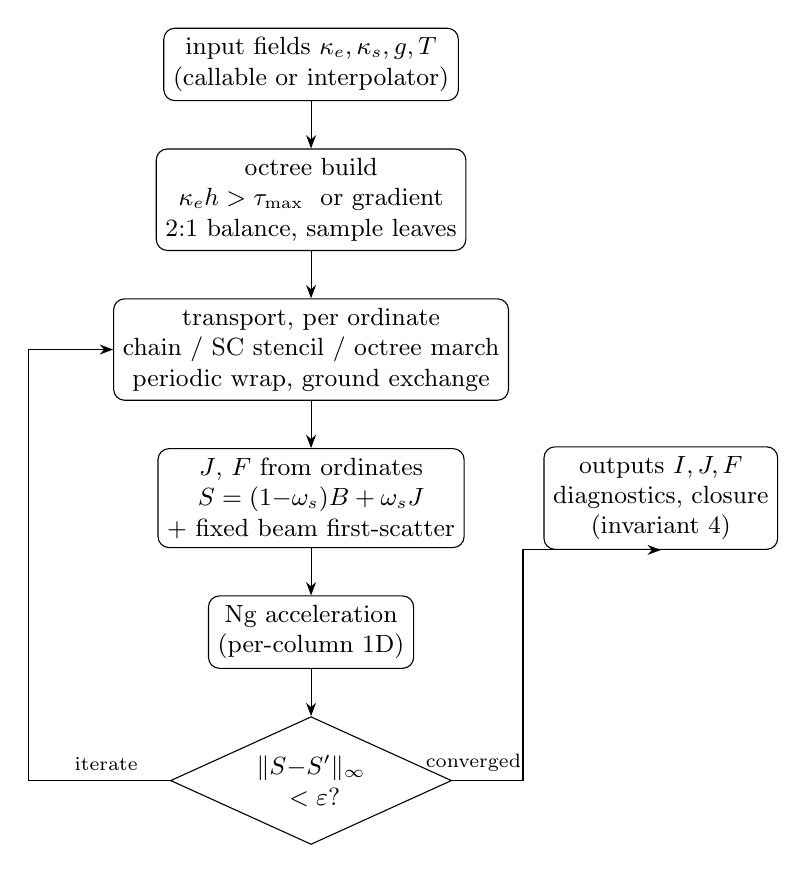
\begin{tikzpicture}[scale=.9, every node/.style={font=\small}]
  \node[draw, rounded corners, align=center] (in)
       {input fields $\ke,\ks,g,T$\\(callable or interpolator)};
  \node[draw, rounded corners, align=center, below=6mm of in] (oct)
       {octree build\\$\ke h>\tau_{\max}$ \ or\ gradient\\2:1 balance, sample leaves};
  \node[draw, rounded corners, align=center, below=6mm of oct] (sweep)
       {transport, per ordinate\\chain / SC stencil / octree march\\
        periodic wrap, ground exchange};
  \node[draw, rounded corners, align=center, below=6mm of sweep] (src)
       {$J$, $F$ from ordinates\\ $S=(1{-}\omega_s)B+\omega_s J$\\
        $+$ fixed beam first-scatter};
  \node[draw, rounded corners, align=center, below=6mm of src] (acc)
       {Ng acceleration\\(per-column 1D)};
  \node[draw, diamond, aspect=2.2, align=center, below=6mm of acc] (conv)
       {$\|S{-}S'\|_\infty$\\ ${}<\varepsilon$?};
  \node[draw, rounded corners, align=center, right=10mm of src] (out)
       {outputs $I,J,F$\\diagnostics, closure\\(invariant 4)};
  \draw[-{Stealth}] (in) -- (oct);
  \draw[-{Stealth}] (oct) -- (sweep);
  \draw[-{Stealth}] (sweep) -- (src);
  \draw[-{Stealth}] (src) -- (acc);
  \draw[-{Stealth}] (acc) -- (conv);
  \draw[-{Stealth}] (conv.west) -- ++(-2.0,0)
    node[above,font=\scriptsize,pos=.45,sloped] {iterate} |- (sweep.west);
  \draw[-{Stealth}] (conv.east) -- ++(1.0,0) node[above,font=\scriptsize,pos=.3]
    {converged} |- (out.south);
\end{tikzpicture}
\caption{The SC solver loop (lambda iteration with Ng acceleration),
structured like DOIT: incoming radiation is transported, the source is
rebuilt, then the next iteration. The beam first-scatter source is a
fixed input, never iterated.}
\label{fig:flow}
\end{figure}

%=============================================================================
\section{Iteration: lambda iteration and Ng acceleration}
\label{sec:iteration}
%=============================================================================

The iteration loop is plain lambda iteration with the scattering integral
evaluated on the quadrature (one BLAS matmul per $g$-bucket per
iteration), accelerated by one-dimensional Ng recursion per vertical
column. Figure~\ref{fig:ng} shows histories for a conservative case
(isotropic slab, $\omega_s=0.99$): Ng cuts 231 iterations to 16, both
runs reaching the same fixed point. The fixed-point agreement pinned in
T1 is a cloud-case measurement: $\Delta J/J=3.8\cdot10^{-7}$ against a
$10^{-5}$ band. On
the cloud case itself Ng is \emph{not} a wall-time win (finding F6 ---
iteration counts are pinned; the gate asserts only that Ng does not
pathologically slow the solve). Convergence tolerance in the matrix runs
is $10^{-8}$ on the plain-iteration residual of the swept source.

\begin{figure}[htbp]
\centering
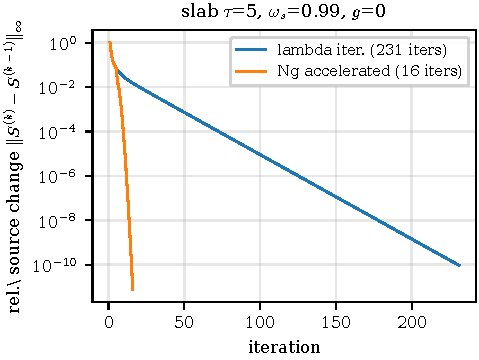
\includegraphics[width=.48\textwidth]{fig_ng.pdf}
\caption{Source-change histories, slab $\tau=5$, $\omega_s=0.99$:
lambda iteration vs 1D Ng acceleration; both runs converge to the same
fixed point (T1 pins the cloud-case agreement at
$\Delta J/J=3.8\cdot10^{-7}$, band $10^{-5}$).}
\label{fig:ng}
\end{figure}

%=============================================================================
\section{Monte Carlo family}
\label{sec:mc}
%=============================================================================

The MC family (\texttt{rt3d/mc/}) is an independent implementation that
shares only geometry, input sampling, and the ground law. It supplies the
zero-noise and statistical cross-checks that make the SC family's
structure trustworthy.

\subsection{Null-collision tracking}

Transport uses Woodcock (null-collision) tracking with a majorant
$\ke^{\max}$ over cell or global mode: candidate interaction points are
sampled from the majorant exponential and thinned against the true local
$\ke$. The same tracker drives deterministic line integrals (used for the
exact cross-family identities), next-flight radiance estimators, and
analog flights. HG directions are sampled from the analytic CDF with
exact normalization --- in contrast to the SC quadrature normalization of
the beam first-scatter term, which is the origin of finding F14. Segment
marching shares the octree walker; one MC bug found by the gate (F12:
uninitialized face-crossing times for axis-parallel directions) is
documented in section~\ref{sec:findings}.

\subsection{Solver A: forward two-stage}

\emph{Stage 1} computes the mean intensity $J$ (and hence the local source
$S=(1-\omega_s)B+\omega_s J$) with one of two estimators:
a lambda-iteration variant (fresh or common-random-number photon streams,
optional Ng) and an \emph{explicit} generation-based variant (analog
collision chains, first scatter of the beam and of boundary/ground
sources sampled as fixed populations). Stage 1 is a $J$-only solver: it
has no angular quadrature, so comparisons to SC use $J_{\mathrm{total}}$
(collided plus \emph{tallied or analytic} uncollided beam column --- a
convention that must be matched before differencing; see
section~\ref{sec:findings}, interpretation rules).
\emph{Stage 2} produces per-ordinate radiance $I(\Om_i)$ from the frozen
source, either by a deterministic march fed the SC's own $\delta$-M
source --- which reproduces the SC sweep to $10^{-12}$ (tier T2, the
family-crossing identity) --- or by next-flight estimators with
per-cell/per-ordinate variance bookkeeping.

\subsection{Solver B: backward (adjoint) MC}

For detector problems, histories are traced \emph{backwards} from a probe
point (or from a quadrature ordinate in the all-sky mode, where the adjoint
cone replaces the detector) through emission, scattering, boundaries, and
ground reflections, weighting each collision by the adjoint path
contribution. The all-sky mode compares per-ordinate columns against the
SC solution; deviations are noise-limited only after the F3 variance mask
and are otherwise limited by the F14 quadrature convention.

\subsection{Ground, sources, and variance reduction}

The MC ground law \eqref{eq:ground} was implemented in phase M6 and closes
finding F1: all families support the Lambertian/emissive ground, including
reflected-beam populations and adjoint ground cones (suite M6, 13 tests
against closed forms). Sources enter as separate populations: top-boundary
inflow, beam first scatter, ground emission/reflection; batch statistics
are tracked per population and merged. Variance reduction includes
common random numbers (valid only for homogeneous fields, F5) and
stratified population sampling. Error accounting follows
section~\ref{sec:validation}: per-cell batch $\sigma$ is honest per cell
(F9) but aggregate domain error must come from seed splitting, never from
quadrature of the per-cell $\sigma$.

\begin{figure}[htbp]
\centering
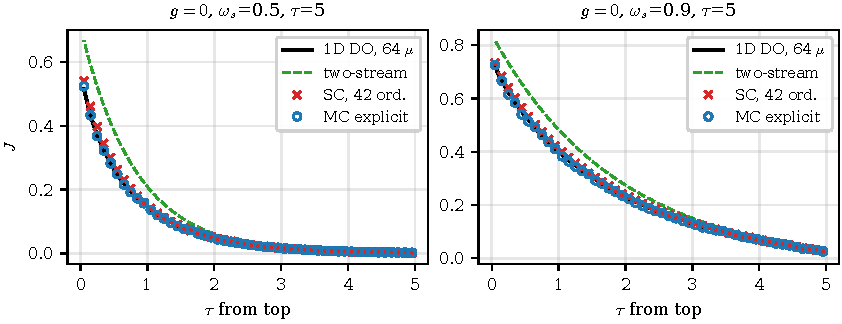
\includegraphics[width=.85\textwidth]{fig_mc_slab.pdf}
\caption{MC stage-1 $J$ on the 1D slab ($\tau=5$, $g=0$) against the
1D discrete-ordinates reference (64 Gauss--Legendre $\mu$) and the
two-stream closure, together with the SC solver (42 ordinates). MC bands
are $2\sigma$ history-batch bands; MC transport is angle-exact, so the
visible deviation from the 1D reference is the reference's own cell
discretization plus statistical noise.}
\label{fig:mcslab}
\end{figure}

%=============================================================================
\section{Validation architecture}
\label{sec:validation}
%=============================================================================

\subsection{Verification invariants}

Five invariants gate every change to transport, source, or iteration code:
(1)~$\sum_i w_i=4\pi$ for the direction grid;
(2)~$\int\Phi\,d\Om=1$ for HG (including MC samplers);
(3)~$\ks=0$, $B=0$ $\Rightarrow$ transmittance $=e^{-\tau}$ along
\emph{every} ray --- asserted \emph{per family} (octree march and chain
exact to $10^{-15}$; the unigrid SC stencil is not, by F11);
(4)~$\nabla\cdot F$ equals the heating rate (energy closure, tested with
an octree-capable closure operator, tier T4);
(5)~the octree result converges to the uniform-grid result for the
Gaussian cloud.

(These five checks were originally called \emph{anchors} throughout the
project; on 2026-11-16 the term was renamed to \emph{verification
invariants} everywhere --- code, gate (\texttt{test\_matrix\_invariants.py}),
docs, plans, and this report. Only pre-rename compiled artifacts
(\texttt{docs/*.pdf}, older PNG figures under \texttt{plot/}) still show
the old term.)

\subsection{Tiers T0--T5 and M6}

The pytest gate (tiers T0--T5) and the report runner
(\texttt{solver\_matrix.py}) share case and statistics helpers, so
they cannot drift apart. Every solver variant of both families runs on one
physical setup (section~\ref{sec:formulation}); correctness is established
against a fine-octree reference rung (REF: $\tau_{\max}=0.5$, depth 5,
50\,380 leaves) and refinement ladders, not pairwise agreement alone.

\begin{table}[htbp]
\centering\footnotesize
\caption{The cross-solver test matrix. Test counts and runtimes as
measured on the pinned environment.}
\begin{tabular}{@{}l>{\raggedright\arraybackslash}p{3.0cm}>{\raggedright\arraybackslash}p{7.9cm}r@{}}
\toprule
tier & file & asserts & tests \\
\midrule
T0 & \texttt{matrix\_invariants} & invariants 1--3 per variant (weights, HG
normalization incl.\ MC samplers, Beer--Lambert on identical rays for
chain/SC/octree/JIT/NumPy/MC cell+global/adjoint/beam-$\tau$) & 43 \\
T1 & \texttt{matrix\_equivalence} & deterministic equivalence: JIT vs NumPy
and threading bit-identical; $\delta$-M orders vs order 0; Ng fixed point;
chain vs SC band; ground/beam/periodic structure; guards & 20 \\
T2 & \texttt{matrix\_crossfamily} & zero-noise identity: MC deterministic
line integral fed the SC source $\equiv$ SC octree sweep (max $1.2\cdot
10^{-12}$); negative control (physical $\ke$ under $\delta$-M fails by
$\ge10^{-2}$); ground stage-2 identity (F13 guard); unigrid pinned as
band (F11) & 13 \\
T3 & \texttt{matrix\_statistics} & statistical consistency under the noise
model: A1 explicit vs $\lambda$, A1 vs SC, seed-pair pooled $z$,
next-flight F3 masking, adjoint masked $z$, all-sky ground MC vs SC & 15 \\
T4 & \texttt{matrix\_closure} & invariant 4 per family: face powers vs
$\int4\pi\ka(B-J)\,dV$, ground-case closure (bottom-face power includes
reflected + emitted parts), cross-family absorbed power & 21 \\
T5 & \texttt{matrix\_ladder} & refinement ladders per family, reference
ranking, order fits, per-family invariant 3, MC $N^{-1/2}$ by seed splitting
& 10 \\
M6 & \texttt{mc\_ground} & MC ground law against closed forms: vacuum
emission, Beer--Lambert + albedo continuum, adjoint cones, reflected-beam
populations, stage-2 vs SC, equal-seed determinism pairings & 13 \\
\bottomrule
\end{tabular}
\end{table}

\subsection{Pinned bands: measured imperfections, not tolerated ones}

Everything the gate asserts numerically is a \emph{measured} threshold: a
regression outside a band fails the gate naming the band. Representative
pinned values (measured values and the bands guarding them):
$\delta$-M~1/2 vs 0 converged-field gap measured
$\le1.5\cdot10^{-2}$ in $J$ and $6\cdot10^{-2}$ in $I$ (= the unigrid
bands); Ng vs plain lambda fixed point measured
$\Delta J/J=3.8\cdot10^{-7}$, band $10^{-5}$; octree march vs SC chain
fed the same source $1.2\cdot10^{-12}$, and vs the solver's own $I$
$\le5\cdot10^{-9}$ at tolerance $10^{-8}$; ground stage-2
identity $8.6\cdot10^{-10}$; unigrid march-vs-chain measured 0.26 in $J$
and 0.93 in $I$, pinned bands 0.35/1.2 ---
pinned as an \emph{F11 finding}, not asserted as correctness. The capability
matrix (Table~\ref{tab:capability}) records which configuration each
variant supports; after phase M6 the only unsupported configuration is the
variable-height ground.

\begin{table}[htbp]
\centering\small
\caption{Capability matrix after phase M6 (finding F1 closed).}
\label{tab:capability}
\resizebox{\textwidth}{!}{\begin{tabular}{@{}llcccccc@{}}
\toprule
feature & \multicolumn{3}{c}{SC family} & \multicolumn{3}{c}{MC family} \\
\cmidrule(lr){2-4}\cmidrule(lr){5-7}
 & chain & unigrid SC & octree & A1 stage-1 & A2 stage-2 & adjoint B \\
\midrule
thermal emission $B$ & yes & yes & yes & yes & yes & yes \\
solar beam & yes & yes & yes & yes & yes & yes \\
Lambertian ground & yes & yes & yes & yes (M6) & yes (ground\_I) & yes (M6) \\
variable-height ground & n/a$^\dagger$ & n/a$^\dagger$ & n/a$^\dagger$ & n/a$^\dagger$ & n/a$^\dagger$ & n/a$^\dagger$ \\
angular quadrature & 42--642 & 42--642 & 42--642 & none & binning & exact HG \\
energy closure (invariant 4) & yes & yes & yes (octree) & n/a ($J$ only) & yes (stage-2 $I$) & n/a (detector) \\
\bottomrule
\end{tabular}
}
\medskip
{\footnotesize $^\dagger$ guarded by \texttt{NotImplementedError} in both
families; the only unsupported configuration anywhere in the matrix.}
\end{table}

%=============================================================================
\section{Results and findings}
\label{sec:results}
%=============================================================================

\subsection{Transport behavior on the matrix case}

Figure~\ref{fig:beerk} is the invariant-3 statement in two panels, run on
a single transverse column: there the chain's cell-to-cell path is also
the true ray path, so chain and octree march reproduce pure-absorber
attenuation to floating-point precision for all 42 ordinates, while the
SC stencil already deviates. On grids with transverse extent the chain's
path stops being the true ray, and the same grazing-ordinate-dominated,
$h$-independent error appears in \emph{both} unigrid schemes (finding
F11), which is also why unigrid variants plateau at $\approx4\%$ rms $J$
away from the octree reference at every resolution.

\begin{figure}[htbp]
\centering
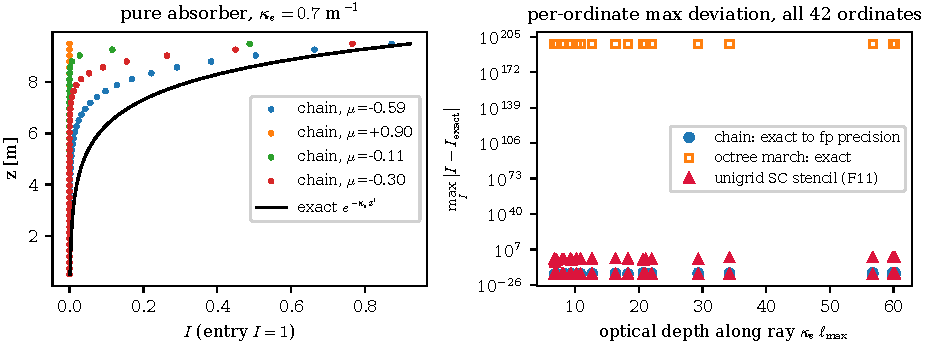
\includegraphics[width=.95\textwidth]{fig_beer_f11.pdf}
\caption{Invariant 3 and finding F11, on a single transverse column
(where even the chain path is the true ray). Left: Beer--Lambert attenuation for
sample chain characteristics ($\ke=0.7$\,m$^{-1}$, top inflow $I=1$)
against the analytic law. Right: per-ordinate maximum deviation from the
exact solution vs ray optical depth, all 42 ordinates: chain and octree
march sit at the floating-point floor; the unigrid SC stencil deviates
by up to $10^{-1}$, with the worst ordinates the grazing ones (F11 ---
on transverse grids the chain carries an $h$-independent error of its
own, $\approx12\%$ rms: Table~\ref{tab:findings},
Figs.~\ref{fig:jmaps} and~\ref{fig:ranking}; pinned as a finding, the
solver was left unchanged).}
\label{fig:beerk}
\end{figure}

Figures~\ref{fig:slab} and \ref{fig:toa} show the classical 1D slab check
(the 3D solver at 42 ordinates follows a 64-$\mu$ 1D discrete-ordinates
reference with deviations well below the two-stream closure error) and the
plane-parallel TOA upward-radiance spectrum for the full 3D all-sky case
(42-ordinate unigrid SC visibly biased at small $\mu$; octree tracks the
642-ordinate reference closely).

\begin{figure}[htbp]
\centering
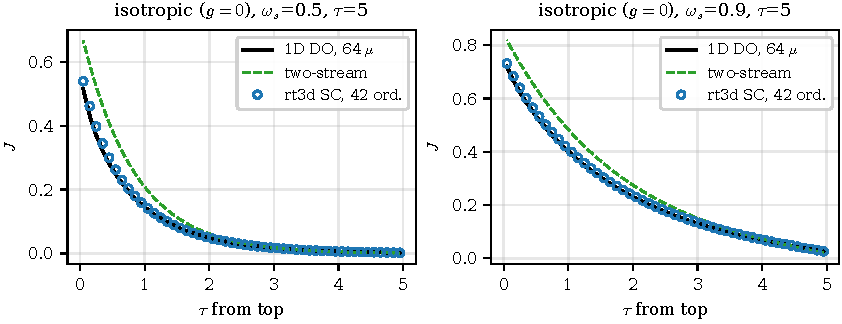
\includegraphics[width=.85\textwidth]{fig_slab.pdf}
\caption{Phase-2 slab validation: 3D SC solver (42 ordinates) vs 1D DO
reference (64 Gauss--Legendre $\mu$ levels) vs two-stream, isotropic
scattering, $\tau=5$, $\omega_s=0.5$ and 0.9.}
\label{fig:slab}
\end{figure}

\begin{figure}[htbp]
\centering
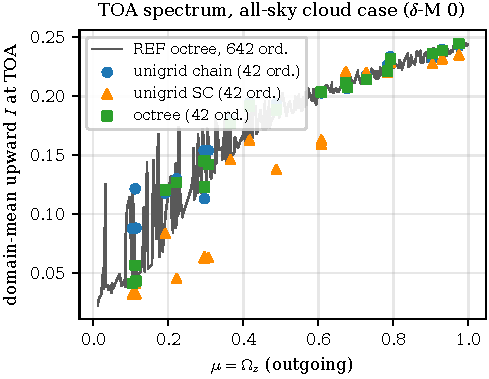
\includegraphics[width=.5\textwidth]{fig_toa.pdf}
\caption{Domain-mean upward radiance at top of atmosphere vs outgoing
$\mu$, all-sky cloud case ($\delta$-M 0): 42-ordinate unigrid chain,
unigrid SC, and octree variants against the 642-ordinate octree
reference. The unigrid SC bias at small $\mu$ is the F11 stencil error
seen at grazing exit angles.}
\label{fig:toa}
\end{figure}

\subsection{Accuracy ranking against the reference}

Table~\ref{tab:matrix} lists every matrix run; Figs.~\ref{fig:jmaps} and
\ref{fig:ranking} give the field structure and the error ranking. The
octree ladder reaches $4\cdot10^{-3}$ rms $J$ against REF at depth 5
($\tau_{\max}=1$); REF's own residual error, bounded by a depth-7 yardstick
rung, is $5.5\cdot10^{-3}$ rms --- the ladder saturates at the
$\tau$-saturation floor (F10). Unigrid variants sit at the F11 plateau.
The JIT and threaded paths are bit-identical to the NumPy reference
(their rows are omitted from the ranking figure).

\begin{table*}[htbp]
\centering
\resizebox{\textwidth}{!}{\begin{tabular}{llrrrrrr}
\toprule
variant & grid & cells & iters & wall [s] & $\overline{J}$ &
closure & rms $J$ err vs REF \\
\midrule
u12/chain & unigrid & 1,728 & 23 & 0.15 & 0.88774 & 5.795e-02 & 4.020e-02 \\
u24/chain & unigrid & 13,824 & 15 & 0.61 & 0.89230 & 8.679e-02 & 4.412e-02 \\
u48/chain & unigrid & 110,592 & 17 & 5.64 & 0.89344 & 9.203e-02 & 4.368e-02 \\
u24/sc & unigrid & 13,824 & 19 & 0.99 & 0.78691 & -3.261e-01 & 1.054e-01 \\
u24/chain/jit-false & unigrid & 13,824 & 15 & 0.62 & 0.89230 & 8.679e-02 & 4.412e-02 \\
u24/chain/njobs1 & unigrid & 13,824 & 15 & 0.62 & 0.89230 & 8.679e-02 & 4.412e-02 \\
oct-d2(tau2)/chain & octree\_grid & 6,952 & 16 & 2.54 & 0.86454 & -3.508e-03 & 2.050e-02 \\
oct-d3(tau2)/chain & octree\_grid & 25,264 & 16 & 8.4 & 0.86479 & -2.239e-03 & 5.856e-03 \\
oct-d5(tau1)/chain & octree\_grid & 34,476 & 16 & 13.04 & 0.86424 & -3.256e-04 & 4.189e-03 \\
oct-REF/ng-off & octree\_grid & 50,380 & 16 & 21.23 & 0.86424 & 4.200e-03 & 3.496e-10 \\
oct-REF/dM2 & octree\_grid & 50,380 & 21 & 25.88 & 0.86421 & 3.653e-03 & 1.604e-04 \\
oct-REF/chain & octree & 50,380 & 16 & 19.72 & 0.86424 &  & 0 (ref) \\
A1/explicit & octree-d2 & 6,952 & 1 & 5.65 & 0.74929 & -- & -- \\
A1/lambda & octree-d2 & 6,952 & 100 & 228.28 & 0.74934 & -- & -- \\
A1/explicit/global & octree-d2 & 6,952 & 1 & 6.62 & 0.74999 & -- & -- \\
A2/next-flight & octree-d2 & 6,952 & 1 & 0.0 & 0.70858 & -- & -- \\
B/adjoint-all-sky & octree-d2 & 2 & 1 & -- &  & -- & -- \\
\bottomrule
\end{tabular}
}
\caption{Solve matrix (all-sky case, 42 ordinates unless noted). Closure
is the relative invariant-4 residual. Errors are vs the REF solve
($\tau_{\max}=0.5$, depth 5).}
\label{tab:matrix}
\end{table*}

\begin{figure}[htbp]
\centering
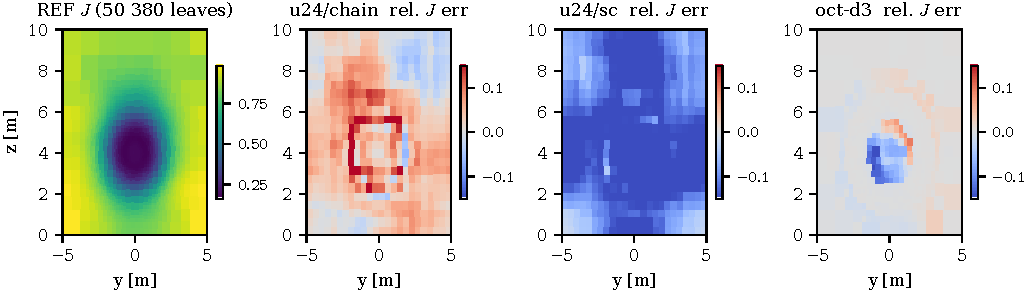
\includegraphics[width=.98\textwidth]{fig_jmaps.pdf}
\caption{Matrix case on the plane $x=0$: REF $J$ (50\,380-leaf octree)
and relative $J$ error of two unigrid variants and one octree rung,
drawn as exact cell/leaf rectangles. The unigrid chain error is dominated
by the F11 grazing-ray structure; the unigrid SC error is larger and
directional; the octree error concentrates at the cloud core. The REF
panel is itself left--right asymmetric by $\approx2\%$ rms ($\approx5\%$
locally) although the configuration is $y$-symmetric: the rotated
42-ordinate direction grid is not $y$-mirror symmetric, so this is a
quadrature-orientation imprint --- angular, not transport, error
(a mirrored direction set reproduces the mirrored field to 0.1\% rms,
and 642 ordinates reduce the asymmetry to $\approx0.2\%$ rms).}
\label{fig:jmaps}
\end{figure}

\begin{figure}[htbp]
\centering
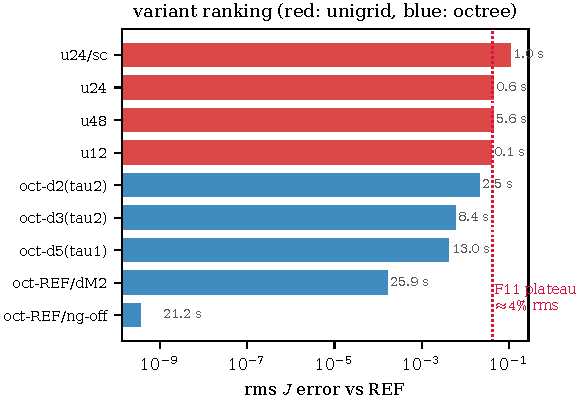
\includegraphics[width=.5\textwidth]{fig_ranking.pdf}
\caption{Ranking of all deterministic variants by rms $J$ error vs REF
(log scale; wall time annotated). Red: unigrid (F11 plateau at
$\approx4\cdot10^{-2}$ for the chain family); blue: octree rungs, which
reach the REF self-noise level. Bit-identical JIT/threading duplicates
omitted.}
\label{fig:ranking}
\end{figure}

Figure~\ref{fig:ladders} summarizes the three convergence ladders: the
unigrid Cauchy ladder is internally textbook first order (fitted slope
1.01), the octree $\tau$-ladder converges in $\tau_{\max}$ with slope
$\approx0.6$ toward the saturation floor, and the MC power error follows
the $N^{-1/2}$ law (seed-split estimate; slope $-0.37$ over three
ladder rungs at modest sample counts --- the gate's dedicated T5 test
measures $N^{-0.49}$).

\begin{figure}[htbp]
\centering
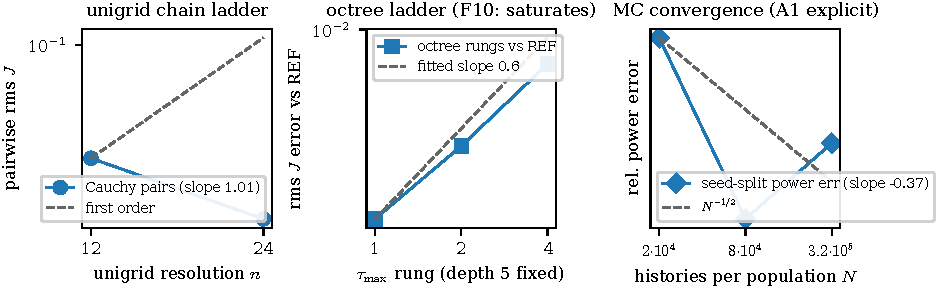
\includegraphics[width=.98\textwidth]{fig_ladders.pdf}
\caption{Refinement ladders. Left: unigrid Cauchy pairs (fitted slope
1.01 in $h$). Middle: octree $\tau_{\max}$ rungs vs REF at fixed depth 5
(slope 0.6, saturating --- F10). Right: MC absorbed-power error by seed
splitting vs $N^{-1/2}$.}
\label{fig:ladders}
\end{figure}

\subsection{Energy closure (invariant 4)}

Figure~\ref{fig:closure} plots the invariant-4 residual
$\oint F\cdot dA-\int4\pi\ka B\,dV$ (relative) for every deterministic
variant. The octree family closes to $3\cdot10^{-4}$ at $\tau_{\max}=1$,
and the residual is dominated by the \emph{face-extrapolation} error,
which improves with base-cell size $h_0$, not with depth (finding F7).
The ground-case closure includes reflected and emitted ground power in
the bottom-face term, with a guard that a dropped ground term fails
loudly. Unigrid residuals are the F11 error leaking through the faces
(chain, $+5.8\cdot10^{-2}$ to $+9.2\cdot10^{-2}$ along the ladder) or
the stencil error (SC, $-3.3\cdot10^{-1}$).

\begin{figure}[htbp]
\centering
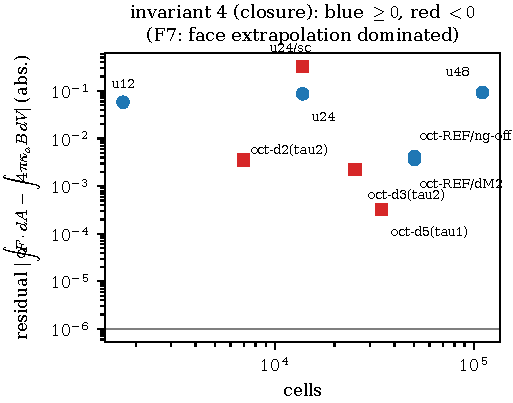
\includegraphics[width=.5\textwidth]{fig_closure.pdf}
\caption{Invariant-4 closure residuals vs problem size (absolute value;
color = sign). The octree ladder improves with $\tau_{\max}$; F7: the
face-extrapolation term, controlled by $h_0$, dominates.}
\label{fig:closure}
\end{figure}

\subsection{Cross-family agreement}

Two statements matter, and they are different in kind.

\emph{Zero-noise identities (T2).} Feeding the MC deterministic march the
SC solver's own source and $\delta$-M extinction reproduces the SC octree
sweep to $1.2\cdot10^{-12}$ (and the solver's own $I$ to
$\le5\cdot10^{-9}$ at tolerance $10^{-8}$), with the ground stage-2
identity at $8.6\cdot10^{-10}$; a negative control (feeding physical
$\ke$ under $\delta$-M) fails the identity by $\ge10^{-2}$, proving the
test can fail. Anything above $10^{-6}$ in a same-grid, same-source
comparison is a bug --- that rule is exactly how F13 was found.

\emph{Statistical comparisons (T3).} On the full all-sky case, MC stage-1
absorbed power sits $-2.35\%$ (A1 explicit, local majorant), $-2.41\%$
(A1 lambda), and $-1.81\%$ (global majorant) from SC on the same grid
(Fig.~\ref{fig:mcpower}); the pinned all-sky band is
$[-5\%,0\%]$ with a coherent quarter-$\sigma$ cell-level offset
contributed partly by F14. The per-cell $z$ statistics are only
meaningful under the F3 mask (Fig.~\ref{fig:zhist},
Table~\ref{tab:mcstats}): unmasked, the next-flight $z$ blows up
(rms 13.9 here; the pinned gate reports up to $10^{25}$ tails) because
per-cell $\sigma$ is zero or undefined where flights never score.

\begin{figure}[htbp]
\centering
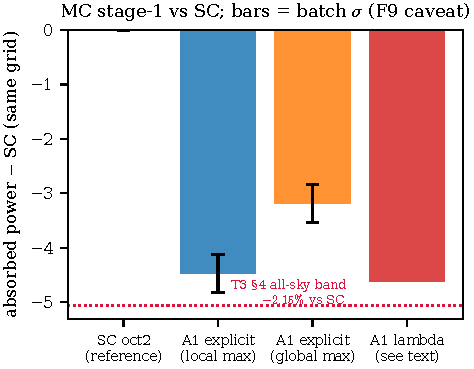
\includegraphics[width=.5\textwidth]{fig_mcpower.pdf}
\caption{MC stage-1 absorbed power vs SC on the same octree grid
(oct-d2), with per-cell batch $\sigma$. All variants sit a few percent
below SC; the dotted line marks the pinned T3 \S4 all-sky band centered
on the measured $-2.15\%$ offset (convention-matched basis: SC $J$ plus
analytic beam column).
Aggregate error bars from per-cell $\sigma$ quadrature are optimistic
2--3$\times$ (F9) --- domain-level statements use seed splitting.}
\label{fig:mcpower}
\end{figure}

\begin{figure}[htbp]
\centering
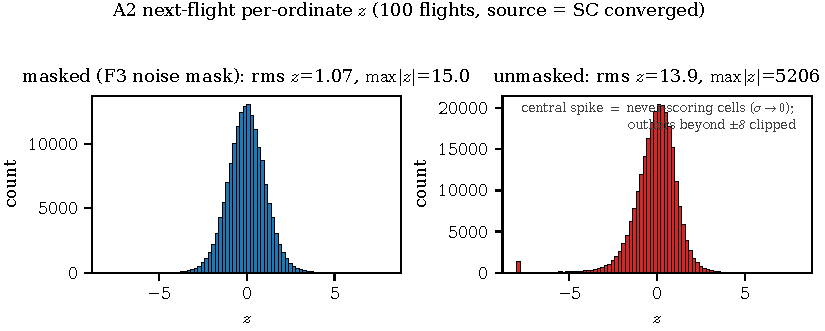
\includegraphics[width=.85\textwidth]{fig_zhist.pdf}
\caption{The F3 story: per-ordinate $z$ of the A2 next-flight estimator
against the deterministic solution with the same converged source. Left:
with the F3 noise mask, the distribution is clean (rms $z\approx1.07$).
Right: unmasked, never-scoring cells stack at $z=0$ and undefined-$\sigma$
outliers (up to $|z|\approx5\cdot10^{3}$ here) wreck the statistic.}
\label{fig:zhist}
\end{figure}

\begin{table}[htbp]
\centering\scriptsize
\caption{Pinned $z$-statistics (gate report, oct-d2 grids; see
\texttt{plot/solver\_matrix/mc\_stats.csv}). The adjoint rows carry the
F14 caveat: per-ordinate gaps are angle-limited, not noise-limited.}
\label{tab:mcstats}
\begin{tabular}{llrrrrr}
\toprule
quantity & mask & $n$ & mean $z$ & rms $z$ &
$\{|z|>2\}$ & $\{|z|>3\}$ \\
\midrule
A1 seed pair  (J\_total) & masked & 6952 & -0.016 & 0.635 & 0.0033 & 0.0000 \\
A1 seed pair  (J\_total) & unmasked & 6952 & -0.016 & 0.635 & 0.0033 & 0.0000 \\
A2 next-flight vs det  (100 fl.) & masked & 163797 & 0.030 & 1.114 & 0.0640 & 0.0115 \\
A2 next-flight vs det  (100 fl.) & unmasked & 255382 & -0.444 & 54.938 & 0.0747 & 0.0249 \\
B adjoint all-sky leaf 0 & masked & 21 & -0.701 & 1.619 & 0.1905 & 0.0952 \\
B adjoint all-sky leaf 1 & masked & 21 & -1.588 & 2.181 & 0.2857 & 0.0952 \\
\bottomrule
\end{tabular}

\end{table}

\subsection{\texorpdfstring{$\delta$-M}{delta-M} consistency}

\begin{figure}[htbp]
\centering
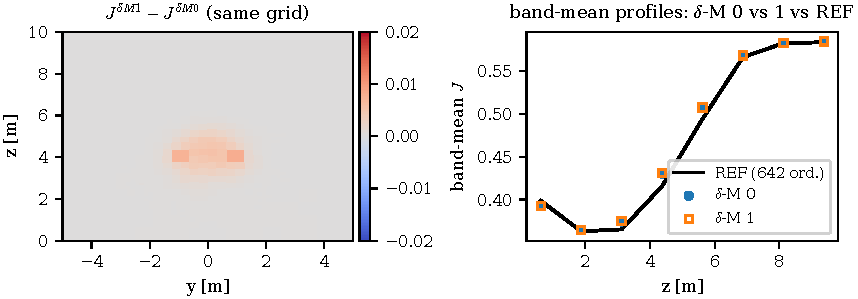
\includegraphics[width=.85\textwidth]{fig_deltaM.pdf}
\caption{$\delta$-M order 1 vs order 0 on the same octree grid (compare
campaign): field difference and band-mean profiles against the
642-ordinate reference. The converged field is nearly $\delta$-M
independent (pinned band $1.5\cdot10^{-2}$ rms $J$), confirming the
$\delta$-M machinery conserves the solution while smoothing the phase
function.}
\label{fig:deltaM}
\end{figure}

\subsection{Findings F1--F14}
\label{sec:findings}

The findings log is part of the gate: each finding is either a fixed bug
with a regression test, a pinned design difference, or an interpretation
rule. Table~\ref{tab:findings} summarizes; the interpretation rules that
follow it are binding for any future number quoted from this project.

\begin{table*}[htbp]
\centering\small
\caption{Findings F1--F14 (findings log, \texttt{docs/solver-matrix.md}).}
\label{tab:findings}
\begin{tabular}{@{}p{0.9cm}p{14.8cm}@{}}
\toprule
ID & finding \\
\midrule
F1 & (closed by M6) MC family used to reject the Lambertian ground; now
supported everywhere. \\
F2 & stage-2 march fed the solver's own source must use
$\ke^{\delta}$ ($\delta$-M) and a direction-resolved source; physical
$\ke$ fails the identity by $\ge10^{-2}$ (negative control, T2). \\
F3 & next-flight per-cell $\sigma$ is invalid (zero/undefined) where
flights never score; every MC-vs-reference $z$ statistic goes through the
noise mask --- unmasked $z$ is meaningless ($10^{25}$ tails observed). \\
F4 & (closed by \S8 of the campaign log) invariant 4 was unigrid-only:
the divergence/closure helpers indexed the unigrid lattice and failed on
octree grids, where the accuracy ranking lives; an octree-capable
closure operator now evaluates invariant 4 for every deterministic
family (T4). \\
F5 & common random numbers couple populations; CRN must stay off for
inhomogeneous fields. \\
F6 & Ng acceleration is not a wall-time win on this cloud; iteration
counts pinned, ``no pathological slowdown'' asserted. \\
F7 & octree closure residual = face-extrapolation error; $h_0$, not depth,
sets closure accuracy. \\
F8 & (guarded, rename pending) two same-named \texttt{heating\_rate}
helpers --- \texttt{diagnostics} (\texttt{kappa\_a, J, B}) and
\texttt{mc.estimators} (\texttt{kappa\_a, B, J}) --- take their arguments
in reversed order; mixing them up flips the sign of every
heating/closure number (this caused a sign bug in the first T4 draft).
The gate now asserts the sign (absorbed power $\le0$ at $B=0$);
aliasing/renaming is the recorded follow-up. \\
F9 & batch $\sigma$ is honest \emph{per cell} (A2 masked rms
$z\approx1.06$ at 100 flights) but the aggregate per-cell $\sigma$
quadrature underestimates whole-domain error 2--3$\times$; aggregate
statements use seed splitting. \\
F10 & the octree's resolution knobs are not interchangeable: the ladder
runs in $\tau_{\max}$ at non-binding depth; the depth ladder saturates;
$h_0$ moves faces, not cell centers. \\
F11 & unigrid chain/SC carry an $h$-independent grazing-ordinate transport
error ($\approx12\%$ rms vs analytic $e^{-\tau}$ in the absorber limit;
octree/march exact to $10^{-15}$). Unigrid plateaus $\approx4\%$ rms $J$
from the octree reference at every resolution. Pinned as a finding;
invariant 3 is asserted per family. \\
F12 & (fixed 2026-11-16) MC segment marcher left face-crossing times
uninitialized for exactly axis-parallel directions ($dy=0$, $z$ poles):
identical seeds gave different runs ($\pm5\%$ power). Fixed
(\texttt{np.full(..., inf)} in \texttt{rt3d/mc/tracking.py}); guarded by
equal-seed pairings at $10^{-12}$. All pre-fix all-sky probe numbers were
artifacts. \\
F13 & (fixed 2026-11-16) stage-2 march and adjoint looked up the ground
column at the \emph{unwrapped} periodic exit point; silent clamping broke
the F2 march identity by $1.2\cdot10^{-1}$ on the ground octree case
(constant ground radiance had hidden it in all unit tests). Fixed by
wrapping \texttt{(x,y)} before the lookup; post-fix identity
$5.6\cdot10^{-17}$/$8.6\cdot10^{-10}$. \\
F14 & (documented design difference) SC normalizes the beam first-scatter
phase function on the direction grid ($\sum_i w_i\Phi_i=1$), MC samples
the analytic HG. On 42 ordinates the raw quadrature defect is 4--8$\times$
at cloud-core $g=0.9$--$0.925$, so beam-case cross-family per-ordinate
comparisons are \emph{angle-limited}, not noise-limited; it contributes to
the $-2.15\%$ all-sky power offset. Direction-grid refinement drives the
conventions together. \\
\bottomrule
\end{tabular}
\end{table*}

Interpretation rules (binding): never difference unmasked MC $z$; never
use per-cell $\sigma$ quadrature for aggregate error; cross-family octree
identities are exact ($>10^{-6}$ means bug); unigrid$\leftrightarrow$octree
gaps of $\approx4\%$ rms $J$ are the F11 plateau; 42-ordinate beam
per-ordinate gaps are F14-limited; MC $J_{\mathrm{total}}$ includes the
uncollided beam while SC $J$ does not (add the analytic column before
differencing --- the $\lambda$ variant never tallies it and reads 8.7\%
low uncorrected); adjoint probe leaves go inside the cloud core, never at
near-vacuum leaves.

%=============================================================================
\section{Performance}
\label{sec:performance}
%=============================================================================

All sweeps vectorize over cells within topological waves or ray blocks;
scattering is one BLAS matmul per $g$-bucket per iteration; ordinates
are embarrassingly parallel (\texttt{n\_jobs} threading, bit-identical to
serial). The Numba fast paths (chain sweep, SC sweep, octree march, MC
tracking) match the NumPy references bit-identically (T1). Wall times on
the matrix case (this machine, 42 ordinates, from Table~\ref{tab:matrix}):
$u24^3$ chain 0.6\,s, $u48^3$ 5.6\,s, octree REF (50\,380 leaves, 16
iterations) 19.7\,s; MC stage-1 A1 explicit (120\,000 histories $\times$
3 populations, 300 batches) 5.7\,s on the oct-d2 grid, i.e.\ MC reaches
SC-level wall time at statistical accuracy on the same grid, while the
$\lambda$-MC variant (100 noisy iterations) costs 228\,s --- the explicit
estimator is the workhorse. The direction grid cost is linear in
$N_{\mathrm{dir}}$: the 642-ordinate reference solve costs roughly
$15\times$ the 42-ordinate one in time and memory, which is why 42
ordinates remains the development grid and 642 is an opt-in flag.

%=============================================================================
\section{Conclusions and known limitations}
\label{sec:conclusions}
%=============================================================================

The project has delivered a working, validated 3D all-sky monochromatic
SC solver (phases 0--6) on an extinction-driven octree with exact
characteristic marches, $\delta$-M, Ng acceleration, and a full
all-sky ground; an independent Monte Carlo family (two-stage forward A1/A2,
adjoint B, Woodcock tracking, MC ground, M6) that cross-validates the SC
family with zero-noise identities at the $10^{-12}$ level and statistical
agreement within measured bands; and a pinned, self-documenting validation
regime (135 tests, tiers T0--T5+M6) in which the two bugs the regime found
(F12, F13) are fixed with regression guards and every remaining
imperfection is a named, measured, interpreted finding.

Known limitations, all documented rather than hidden:
(i)~42 ordinates under-resolve strongly forward-peaked scattering
($g\gtrsim0.5$) and the beam scattering lobe; the convergence study
(42$\to$162$\to$642) quantifies the effect and F14 bounds what
beam-case cross-family comparisons can mean at 42 ordinates.
(ii)~The unigrid transport schemes carry the F11 grazing-ordinate error;
the octree march is the accuracy path.
(iii)~Closure accuracy at faces is set by the octree base cell $h_0$
(F7).
(iv)~The ground is flat; variable-height surfaces raise
\texttt{NotImplementedError} in both families.
(v)~The octree $\tau$-ladder saturates against the reference (F10):
past $\tau_{\max}\approx1$ further $\tau$-refinement buys little, and
REF's own error floor is $\approx5.5\cdot10^{-3}$ rms $J$.
Next steps on the plan are the KOKKOS port of the transport core
(\texttt{plan/kokkos-plan.md}) and production-level direction refinement
(162/642) for publication cases.

%=============================================================================
\appendix
\section{Reproduction}
\label{sec:reproduce}
%=============================================================================

All numbers and figures in this report regenerate from the repository
(miniforge environment \texttt{pyarts}, interpreter by absolute path):

\begin{verbatim}
# test gate (tiers T0-T5 + M6 + per-feature suites)
~/miniforge3/envs/pyarts/bin/python -m pytest -q
~/miniforge3/envs/pyarts/bin/python -m pytest -q -m "not slow"

# solver-matrix report (CSVs + PNG figures under plot/solver_matrix/)
~/miniforge3/envs/pyarts/bin/python scripts/solver_matrix.py

# this report's vector figures and table fragments (report/figures/,
# report/tables/; reuses the caches under plot/*/_solve_cache/ and
# caches its own solves under report/figures/_cache/)
~/miniforge3/envs/pyarts/bin/python scripts/report_figures.py

# LaTeX build of this report
cd report && latexmk -pdf main.tex
\end{verbatim}

\subsection*{Figure provenance}

Method schematics (Figs.~\ref{fig:directions}, \ref{fig:octree},
\ref{fig:stencil}, \ref{fig:subsegments}, \ref{fig:march}) call the
solver's own geometry helpers, so they show the structures the solver
actually uses. Validation and results figures
(Figs.~\ref{fig:beerk}--\ref{fig:deltaM}) are re-solves or cache reads of
the matrix runs: field maps use the pinned REF field from
\texttt{plot/solver\_matrix/\_solve\_cache/} and fresh solves of the
ranked variants (bit-reproducible, cached); compare-campaign figures
(Fig.~\ref{fig:toa}, Fig.~\ref{fig:deltaM}) read the pinned
\texttt{plot/compare\_transport/\_solve\_cache/} runs (42-ordinate
variants and the 642-ordinate reference). The three-dimensional HTML
scene exports of the compare campaign
(\texttt{plot/compare\_transport/scene\_*.html}) cannot be embedded in
print and are referenced in the text only.

\end{document}
